\documentclass{exam}

\usepackage{units} 
\usepackage{graphicx}
\usepackage[fleqn]{amsmath}
\usepackage{cancel}
\usepackage{float}
\usepackage{mdwlist}
\usepackage{booktabs}
\usepackage{cancel}
\usepackage{polynom}
\usepackage{caption}
\usepackage{fullpage}
\usepackage{xfrac}
\usepackage{enumerate}

\newcommand{\degree}{\ensuremath{^\circ}} 
\everymath{\displaystyle}

\printanswers

% \begin{figure}[H]
%   \centering
%   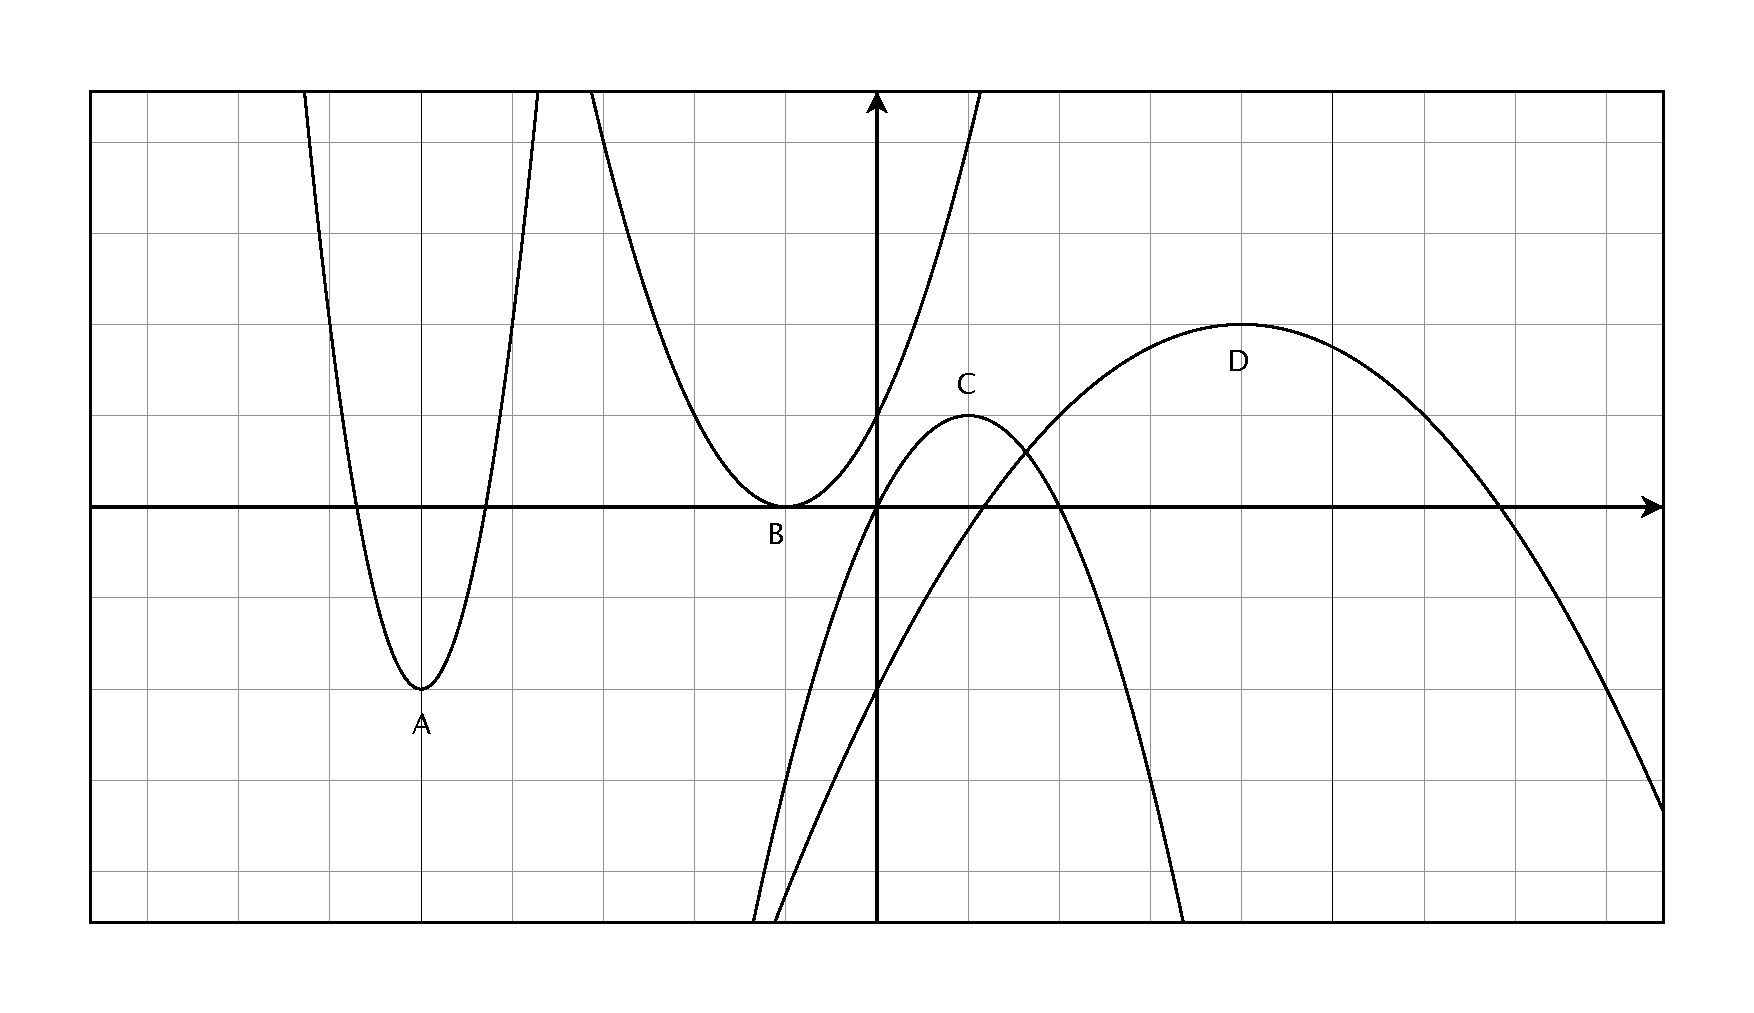
\includegraphics[scale=.3]{problem_7.eps}
%   \caption*{Problem 7}
% \end{figure}

% \begin{tabular}{cc}
% \toprule
% period & amplitude \\
% \midrule
%   $\pi$ & $2$ \\
% \bottomrule
% \end{tabular}

\title{Math 141 Notes \\ Section 4.5}

\date{July 3, 2013}

\begin{document}

  \maketitle
  \tableofcontents

  \section{Homework}
  \begin{enumerate}
    \item
      \[
        \ln 3x^2 = \ln 3 + 2 \ln x \neq 2 \left( \ln 3 + \ln x \right)
      \]
      Only $x$ is squared.

    \item $\log_a a = 1$

  \end{enumerate}

  \section{Population Growth}

  \subsection{Description}
  Just like compound interest: $n(t) = n_0 e^{rt}$.

  \begin{itemize*}
    \item $n$ population at time $t$
    \item $n_0$ initial population
    \item $r$ growth rate--the percentage of the population that produces a new instance each interval
    \item $t$ time
  \end{itemize*}

  \subsection{Examples}

  \begin{enumerate}
    \item bacteria with:
      \begin{itemize*}
        \item $n_0 = 1,000$ 
        \item $r = \unit[0.3]{hr}$; 30\% divide each hour
      \end{itemize*}

      \begin{enumerate}[a]
        \item find the function 
          \[
            n(t) = 1,000 e^{0.3 t}
          \]

        \item how many bacteria after 5 hours? 
          \[
            n(5) = 1,000 e^{0.3 \cdot 5} \approx 4,482
          \]

        \item how many bacteria after 24 hours? 
          \[
            n(24) = 1,000 e^{0.3 \cdot 24} \approx 1,339,430
          \]

        \item how many bacteria were present 2 hours ago? 
          \begin{align*}
            1,000 & = n_0 e^{.3 \cdot 2} \\
            n_0   & \approx 549
          \end{align*}

        \item when did the experiment start with 1 bacterium?
          \begin{align*}
            1,000 & = e^{.3 \cdot t} \\
            t     & \approx \unit[23]{hr}
          \end{align*}

        \item another species propagates at a different rate and reaches 1,000 bacteria in just 8 hours.  What is the
          rate for this species?
          \begin{align*}
            1,000 & = e^{r \cdot 8} \\
            r     & \approx 0.691
          \end{align*}

      \end{enumerate}

    \item 2,000 bacteria; the population doubles every 3 hours
      
      \begin{enumerate}[a]
        \item find the rate:
          \begin{align*}
            2n_0 & = n_0 e^{3r} \\
            r    & = \frac{\ln 2}{3} \\
                 & \approx 0.231 \\
          \end{align*}

        \item how many after 2 hours?
          \[
            n(1) = 2,000 e^{0.231 \cdot 2} \approx 3,175
          \]

        \item when will there be 20,000?
          \begin{align*}
            20,000 & = 2,000 e^{0.231 t} \\
            t      & \approx \unit[9.97]{hr} \\
          \end{align*}

      \end{enumerate}
      
  \end{enumerate}

  \section{Radioactive Decay}

  \subsection{Description}
  Like growth, but with time running backwards: $n(t) = n_0 e^{-rt}$.

  \begin{itemize*}
    \item $n$ quantity at time $t$
    \item $n_0$ initial quantity
    \item $r$ decay rate
    \item $t$ time
  \end{itemize*}

  \subsection{Examples}

  \begin{enumerate}
    \item What is the rate if the half life is $T$ years?
      \begin{align*}
        \frac{n_0}{2} &= n_0 e^{-rT} \\
        -rT           &= \ln \frac{1}{2} \\
        rT            &= \ln 2 \\
        r             &= \frac{\ln 2}{T} \\
      \end{align*}

    \item What is the rate if the half life is 2,000 years?
      \[
        r = \frac{\ln 2}{2,000} \approx 0.000346574 \\
      \]

    \item How old is a sample if 35\% remains and the half life is 2,000 years?
      \begin{align*}
        0.35 n_0 & = n_0 e^{0.000346574 t} \\
        t        & \approx \unit[3,029]{yr} \\
      \end{align*}

    \item How much of an original sample of 100 kg remains after 10,000 years?
      \begin{align*}
        n & = 100 e^{0.000346574 \cdot 10,000} \\
          & \approx \unit[3.125]{kg} \\
      \end{align*}
  \end{enumerate}

\end{document}
